\let\negmedspace\undefined
\let\negthickspace\undefined
\documentclass[journal]{IEEEtran}
\usepackage[a5paper, margin=10mm, onecolumn]{geometry}
\usepackage{tfrupee}

\setlength{\headheight}{1cm}
\setlength{\headsep}{0mm}

\usepackage{gvv-book}
\usepackage{gvv}
\usepackage{cite}
\usepackage{amsmath,amssymb,amsfonts,amsthm}
\usepackage{algorithmic}
\usepackage{graphicx}
\usepackage{textcomp}
\usepackage{xcolor}
\usepackage{txfonts}
\usepackage{listings}
\usepackage{enumitem}
\usepackage{mathtools}
\usepackage{gensymb}
\usepackage{comment}
\usepackage[breaklinks=true]{hyperref}
\usepackage{tkz-euclide}
\usepackage{listings}
\def\inputGnumericTable{}
\usepackage[latin1]{inputenc}
\usepackage{color}
\usepackage{array}
\usepackage{longtable}
\usepackage{calc}
\usepackage{multirow}
\usepackage{hhline}
\usepackage{ifthen}
\usepackage{lscape}

\begin{document}

\bibliographystyle{IEEEtran}
\vspace{3cm}

\title{4.2.6}
\author{EE25BTECH11003 - Adharvan Kshathriya Bommagani}
{\newpage\maketitle}

\renewcommand{\thefigure}{\theenumi}
\renewcommand{\thetable}{\theenumi}
\setlength{\intextsep}{10pt}

\textbf{Question}:\\
Find the direction and normal vectors of each of the following lines.
\begin{enumerate}[label=\textbf{4.2.\arabic*}]
    \setcounter{enumi}{5}
    \item $3x+2 = 0$
\end{enumerate}

\bigskip

\textbf{Solution}:\\

To find the normal and direction vectors for the line $3x+2=0$, we can express the equation in a standard vector form.


The equation of a line can be written in the form $\vec{n}^T \vec{x} = c$, where $\vec{n}$ is the normal vector and $\vec{x} = \myvec{ x \\ y }$.

The given equation can be rewritten to include the $y$ term explicitly:
\begin{align*}
3x + 0y = -2
\end{align*}
This can be expressed in vector form:
\begin{align*}
\myvec{ 3 \\ 0 }^T \myvec{ x \\ y } = -2
\end{align*}
By comparing this to the general form $\vec{n}^T \vec{x} = c$, we can directly identify the \textbf{normal vector} as:
\begin{align*}
\vec{n} = \myvec{ 3 \\ 0 }
\end{align*}


The direction vector $\vec{m}$ is orthogonal (perpendicular) to the normal vector $\vec{n}$. This means their dot product is zero:
\begin{align*}
\vec{m}^T \vec{n} = 0
\end{align*}
Let the direction vector be $\vec{m} = \myvec{ m_1 \\ m_2 }$. We can set up the equation:
\begin{align*}
\myvec{ m_1 & m_2 } \myvec{ 3 \\ 0 } &= 0 \\
(m_1)(3) + (m_2)(0) &= 0 \\
3m_1 &= 0 \\
m_1 &= 0
\end{align*}
Since $m_1 = 0$, the direction vector is of the form $\myvec{ 0 \\ m_2 }$. The vector must be non-zero, so we can choose any non-zero value for $m_2$. The simplest choice is $m_2 = 1$.

Therefore, the \textbf{direction vector} is:
\begin{align*}
\vec{m} = \myvec{ 0 \\ 1 }
\end{align*}

\bigskip

\textbf{Answer:}\\
\textbf{Normal Vector:} $\vec{n} = \myvec{ 3 \\ 0 }$ \\
\textbf{Direction Vector:} $\vec{m} = \myvec{ 0 \\ 1 }$\\



\textbf{Illustration of the Line and Vectors:}
\begin{figure}[h!]
    \centering
    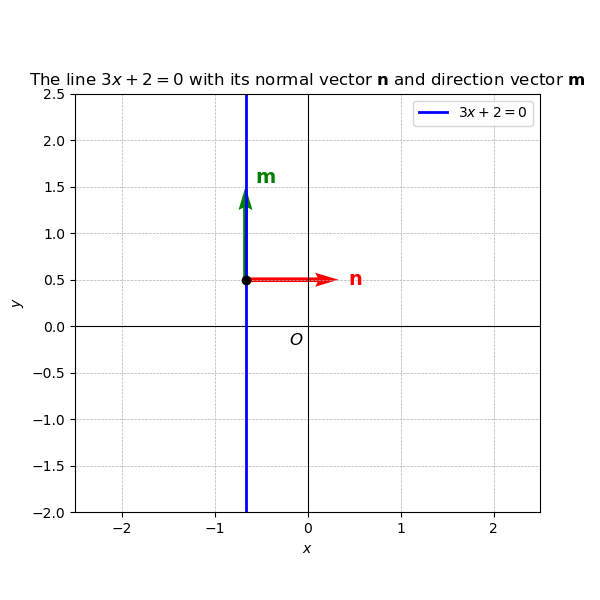
\includegraphics[width=1.0\columnwidth]{figs/fig1.png}
    \caption{Figure for 4.2.6}
    \label{}
\end{figure}

\end{document}